\documentclass[11pt,aspectratio=169]{beamer}
% Change text margins
\setbeamersize{text margin left = 12pt, text margin right = 12pt} 
\setbeamercovered{transparent}

\settowidth{\leftmargini}{\usebeamertemplate{itemize item}}
\addtolength{\leftmargini}{\labelsep}

% \begin{columns} -----------------------------------
\usepackage{arydshln}
\usepackage{multicol}
\usepackage{natbib}
\usepackage{amsmath}
\usepackage{amsfonts}
\usepackage{verbatim}
\usepackage{mathrsfs}
\usepackage{amssymb}
\usepackage{amsthm}
\usepackage{bbm}
\usepackage{bm}
\usepackage{booktabs}
\usepackage{longtable}
\usepackage{multirow}
\usepackage{bigdelim}
\usepackage{makecell}
%\onehalfspacing
\usepackage{courier}
\newcommand{\indicator}[1]{\mathbbm{1}_{\left\{ {#1} \right\} }}

% Title --------------------------------------------
\title{The Welfare Consequences of Rent Controls}
\date{\today}
\author{Shahar Rotberg$^*$ and Lin Zhang$\dagger$ (CMHC)}

\begin{document}

% ------------------------------------------------------------------------------
\begin{frame}
\maketitle
 
 \vspace{1cm}
{\footnotesize $^*$Shahar Rotberg co-authored this paper in his own personal capacity and time. $\dagger$The opinions expressed herein do not necessarily reflect the views of the CMHC.}
\end{frame}

\begin{frame}{Introduction}{Why should we care?}

\vspace{-0.75cm}

\begin{itemize}
    \item Many cities worldwide aim to keep rental housing affordable using rent control policies 
\end{itemize}     

\end{frame}

\begin{comment}
    
\begin{frame}{Introduction}{Why should we care?}

\vspace{-0.75cm}

\begin{itemize}
    \item Why do we need rent control? Can't contracts arise in free market?
    \item First, it's not common to see this in free markets
    \item Second, low-income households need rent control the most, but:
    \begin{itemize}
        \item May have limited bargaining power relative to landlords who do such deals over and over
        \item May have limited knowledge of their rights
        \item May be unable to afford upfront costs to sign agreements to protect them from rent increases:
        \begin{itemize}
            \item Contracts are expensive to prepare
            \item May require substantial initial lump sum payment to landlord to make it profitable for them
        \end{itemize}
    \end{itemize}
\end{itemize}     

\end{frame}

\end{comment}

\begin{comment}
\item Two forms of rent control are most commonly used: unit control and tenancy control
    \begin{itemize}
        \item Unit control: restricts rent hikes during a tenancy as well as when tenants change
        \item Tenancy control: limits rent hikes during tenancy, but can reset rents upon tenant turnover
    \end{itemize}
        \item Literature examined unit control, but left tenancy control under-studied, especially in GE
    \item We develop first GE theory of tenancy control and:
    \begin{itemize}
        \item Nest both rent control policies in a GE housing model
        \item Compare welfare consequences of these two forms of rent control
        \item Calibrate model to data from Toronto, where tenancy control is adopted
    \end{itemize}
    \item Our main findings:
        \begin{itemize}
            \item Moving from tenancy control to unit control: $\downarrow$ welfare and $\downarrow$ allocation of controlled units
            \item Welfare-maximizing to have 65\% of rental market under tenancy control
        \end{itemize}
\end{comment}

%%%%%%%%%%%%%%%%%%%%%%%%%
%%%%%%%%%%%%%%%%%%%%%%%%%
\begin{frame}{Introduction}{Classic view of rent control (unit control)}

\begin{columns}[T]
\begin{column}{0.6\textwidth}
\hspace*{-0.4cm}
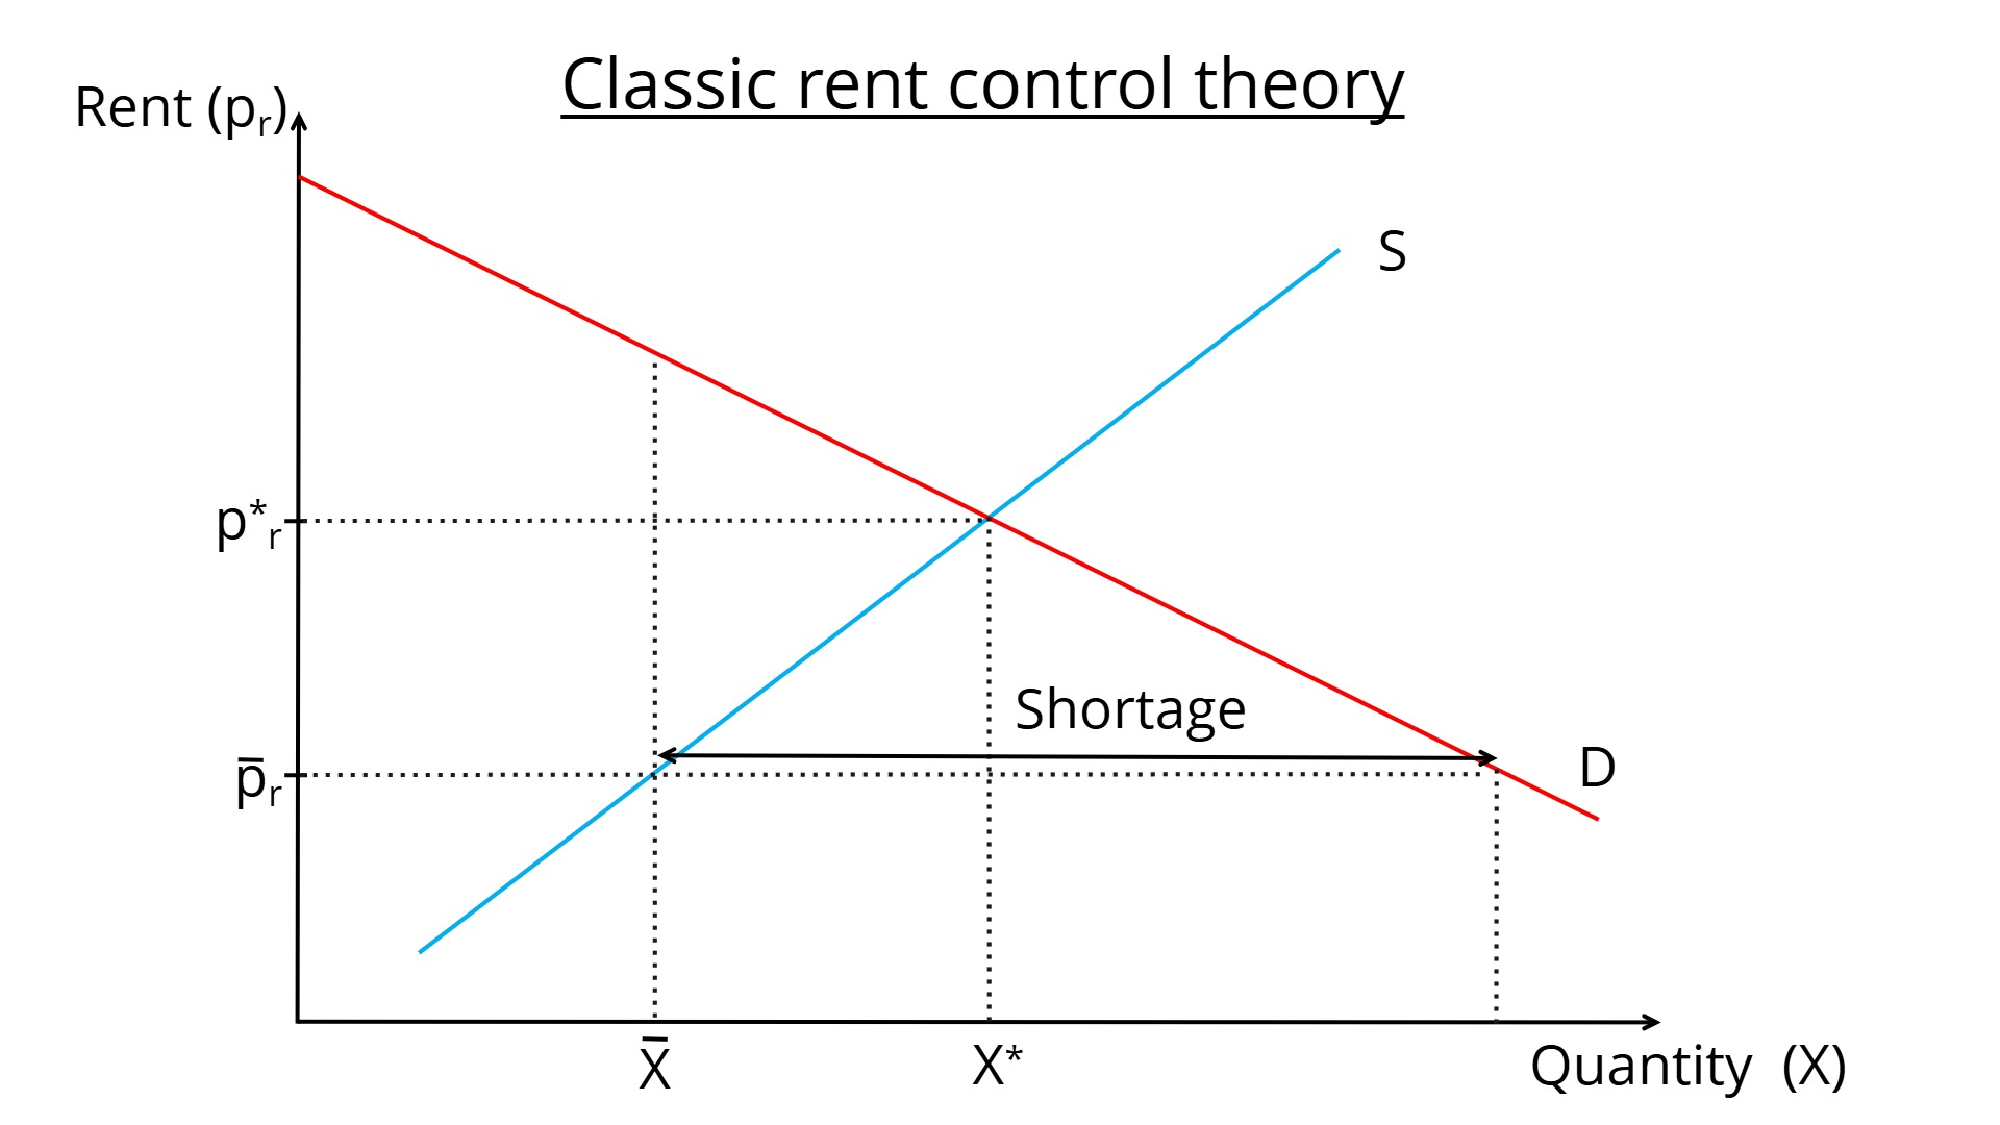
\includegraphics[width=1.4\textwidth]{figures_for_slides/current_lit.pdf}
\end{column}
\begin{column}{0.4\textwidth}
  \begin{itemize}
    \item Rent control is a cap on rent (unit control) $\rightarrow$ shortages $\rightarrow$ lotteries allocate units $\rightarrow$ units do not go to highest WTP $\rightarrow$ misallocation \citep{gl-2003}
    \item This is how it works in New York City, Vancouver, Montréal, Paris 
\end{itemize}     
\end{column}

\end{columns}

\end{frame}

\begin{frame}{Introduction}{Tenancy control}

However:
\begin{itemize}
    \item Many places regulate rents during a tenancy, but let landlords adjust rents upon tenant turnover (tenancy control): Toronto, San Francisco, L.A., D.C., Singapore, Hong Kong
    \item Does this theory apply to tenancy control? 
\end{itemize}

\end{frame}

\begin{frame}{Introduction}{Our general equilibrium theory of tenancy control}

\begin{columns}[T]
\begin{column}{0.6\textwidth}
\hspace*{-0cm}
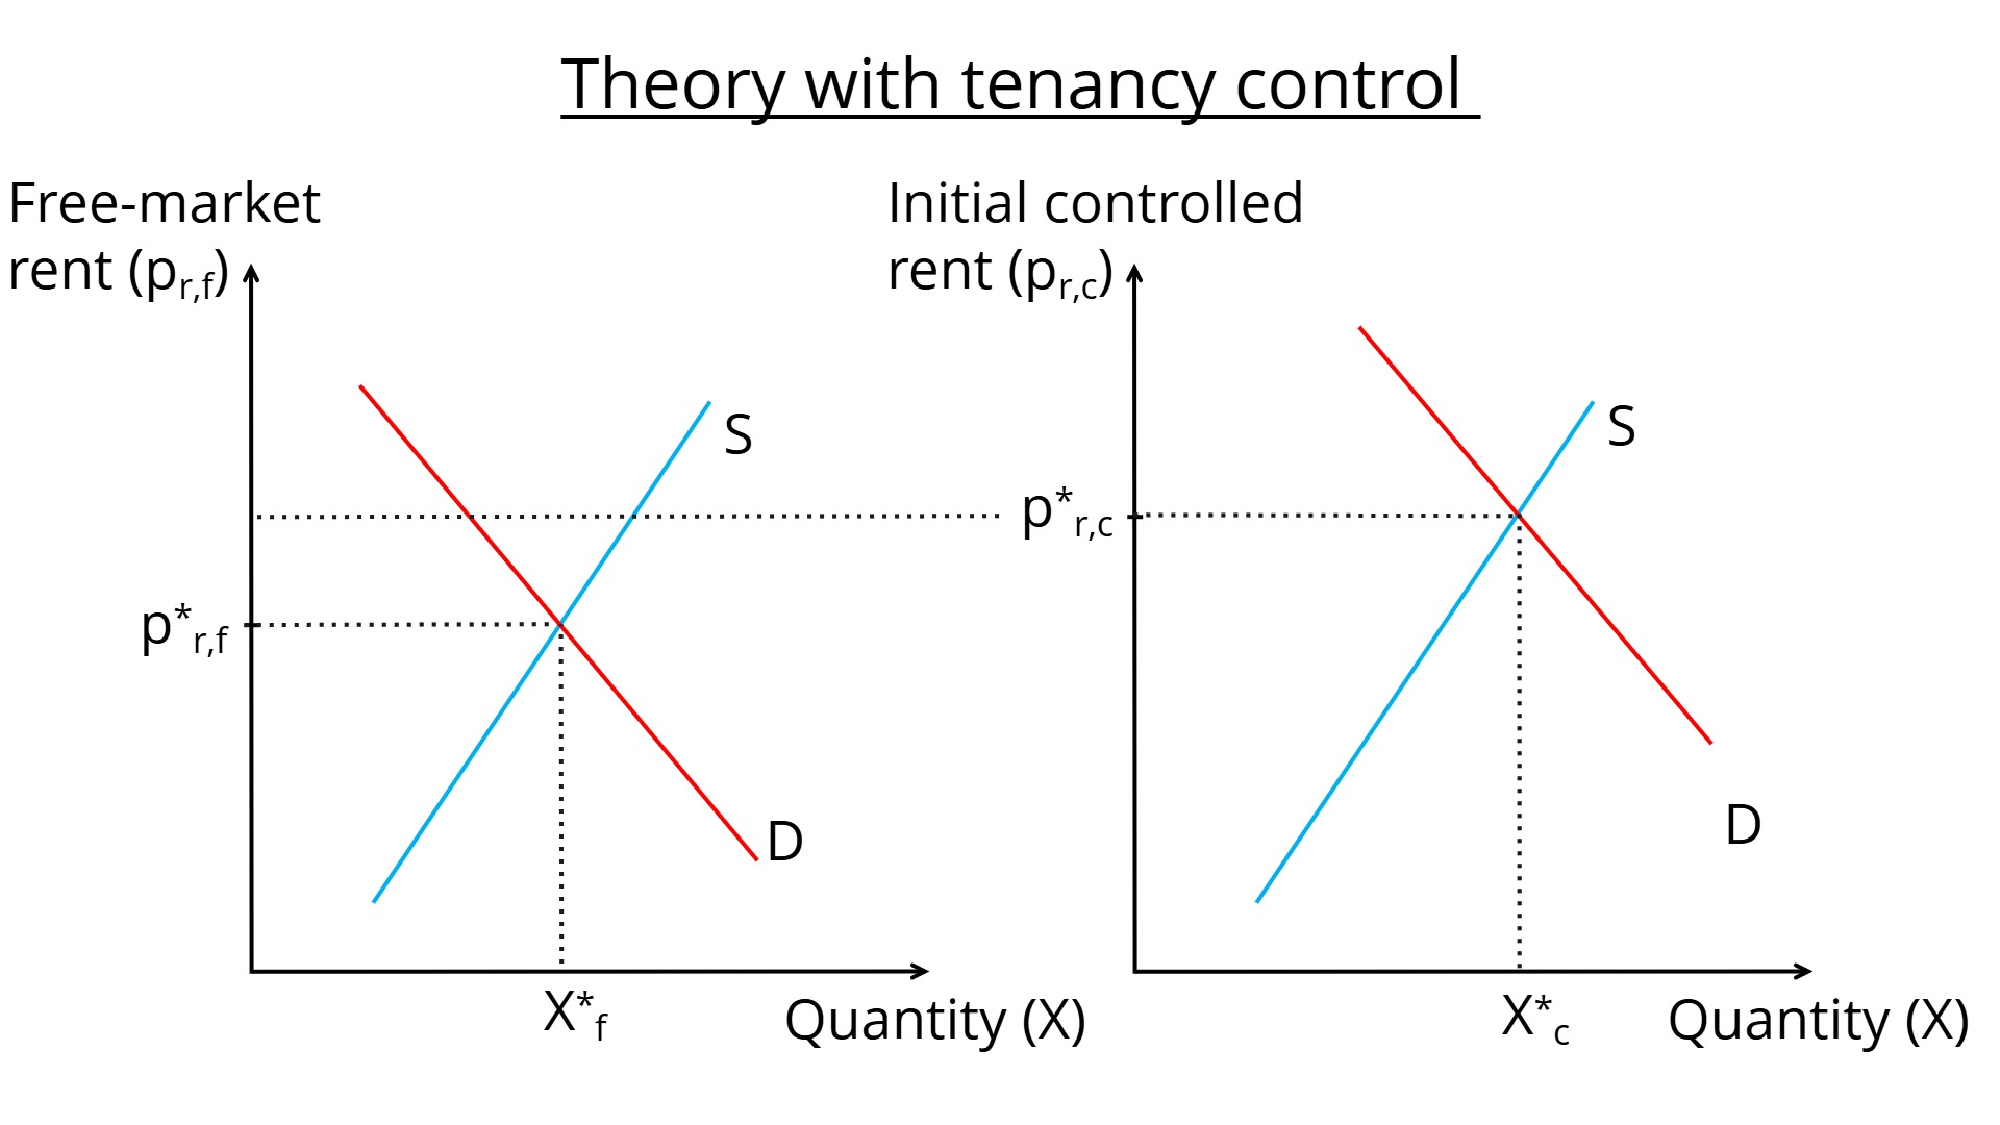
\includegraphics[width=1.3\textwidth]{figures_for_slides/our_theory.pdf}
\end{column}
\begin{column}{0.4\textwidth}
  \begin{itemize}
    \item Competition for controlled units drives up initial controlled rent above free market rents $\rightarrow$ units go to highest WTP $\rightarrow$ no shortages and better allocation
\end{itemize}     
\end{column}

\end{columns}

\end{frame}

\begin{frame}{Introduction}{Unit control vs. tenancy control}

Trade-offs: Time to benefit vs. shortages and allocation
\begin{enumerate}
    \item Unit control provides immediate discounts $\rightarrow$ shortages and misallocation
    \item Tenancy control allocates units via price mechanisms $\rightarrow$ no shortages and better allocation
\end{enumerate}

\vspace{0.5cm}

Price mechanism as tool to improve allocation brought into question with minimum rental size 
\begin{enumerate}
    \item Premium $\rightarrow$ reduces access to low-incomes with highest WTP $\rightarrow$ worse allocation?
\end{enumerate}

\end{frame}

\begin{frame}{Introduction}{Contribution}

In this paper, we develop:
\begin{enumerate}
    \item First general-equilibrium theory of tenancy control
    \item GE model nesting both unit control and tenancy control, calibrated to Toronto
    \item Quant. exercises comparing unit control with tenancy control, and finding optimal control
\end{enumerate}

\end{frame}

{\setbeamercolor{background canvas}{bg=black}
\begin{frame}{}

\centering \Large
\textcolor{white}{Snapshot of results}
    
\end{frame}

}

%%%%%%%%%%%%%%%%%%%%%%%%%
%%%%%%%%%%%%%%%%%%%%%%%%%
\begin{frame}{Snapshot of main results}{Results}

Compared to calibrated benchmark where 70\% of rental market is under tenancy control:
\begin{itemize}
    \item Unit control worsens allocation of controlled units, increases homelessness, and reduces welfare
    \item Full decontrol reduces welfare and increase homelessness
    \item Full tenancy control reduces welfare and marginally reduces homelessness
    \item Welfare-maximizing degree of tenancy control is close to benchmark (65\%)
\end{itemize}

\end{frame}

{\setbeamercolor{background canvas}{bg=black}
\begin{frame}{}

\centering \Large
\textcolor{white}{Road map}
    
\end{frame}

}
    
%%%%%%%%%%%%%%%%%%%%%%%%%
%%%%%%%%%%%%%%%%%%%%%%%%%
\begin{frame}{Road map}

\begin{itemize}
    \item Related literature
    \item Rent control background
    \item Model 
    \item Calibration
    \item Model performance
    \item Experiments
    \item Conclusion and discussion
\end{itemize}

\end{frame}

{\setbeamercolor{background canvas}{bg=black}
\begin{frame}{}

\centering \Large
\textcolor{white}{Related literature}
    
\end{frame}

}

\begin{frame}{Related literature}{}

\begin{itemize}
    \item \citet{gl-2003}: empirically study unit control $\rightarrow$ leads to misallocation
    \item \citet{fallis-1985}: study rent control using static theoretical model
    \item \citet{eric-1995,fmn-2023}: develop GE models of unit control
    \item \citet{diamond-2019}: study expansion of tenancy control in SF, but rents not endogenous
    \item \citet{nagy-1997,early-2000,chen-etal-2016}: show new controlled tenants pay premium
    \item \citet{eo-1998}: show that more rent control reduces homelessness
    \item \citet{abramson-2024,az-2024}: study homelessness in GE, but not its interaction with rent control
\end{itemize}

\end{frame}

{\setbeamercolor{background canvas}{bg=black}
\begin{frame}{}

\centering \Large
\textcolor{white}{Rent control background}
    
\end{frame}

}

\begin{frame}{A timeline of rent control laws in Ontario}
  \centering
     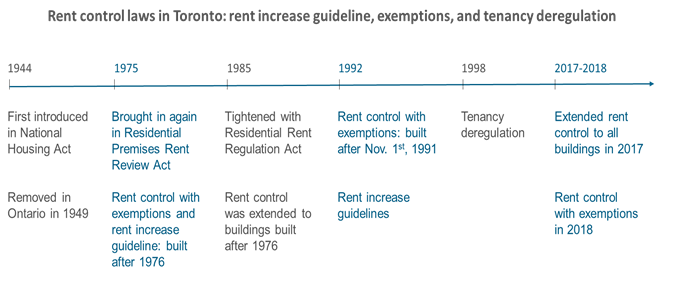
\includegraphics[width=1\textwidth]{figures_for_slides/history_of_rent_control_Toronto.png}
     
\end{frame}

%%%%%%%%%%%%%%%%%%%%%%%%%
%%%%%%%%%%%%%%%%%%%%%%%%%


{\setbeamercolor{background canvas}{bg=black}
\begin{frame}{}

\centering \Large
\textcolor{white}{Model}
    
\end{frame}

}

\begin{frame}{Model at high level}{}
  \centering
  \vspace{-0.2cm}
\hspace*{-0.6cm}
     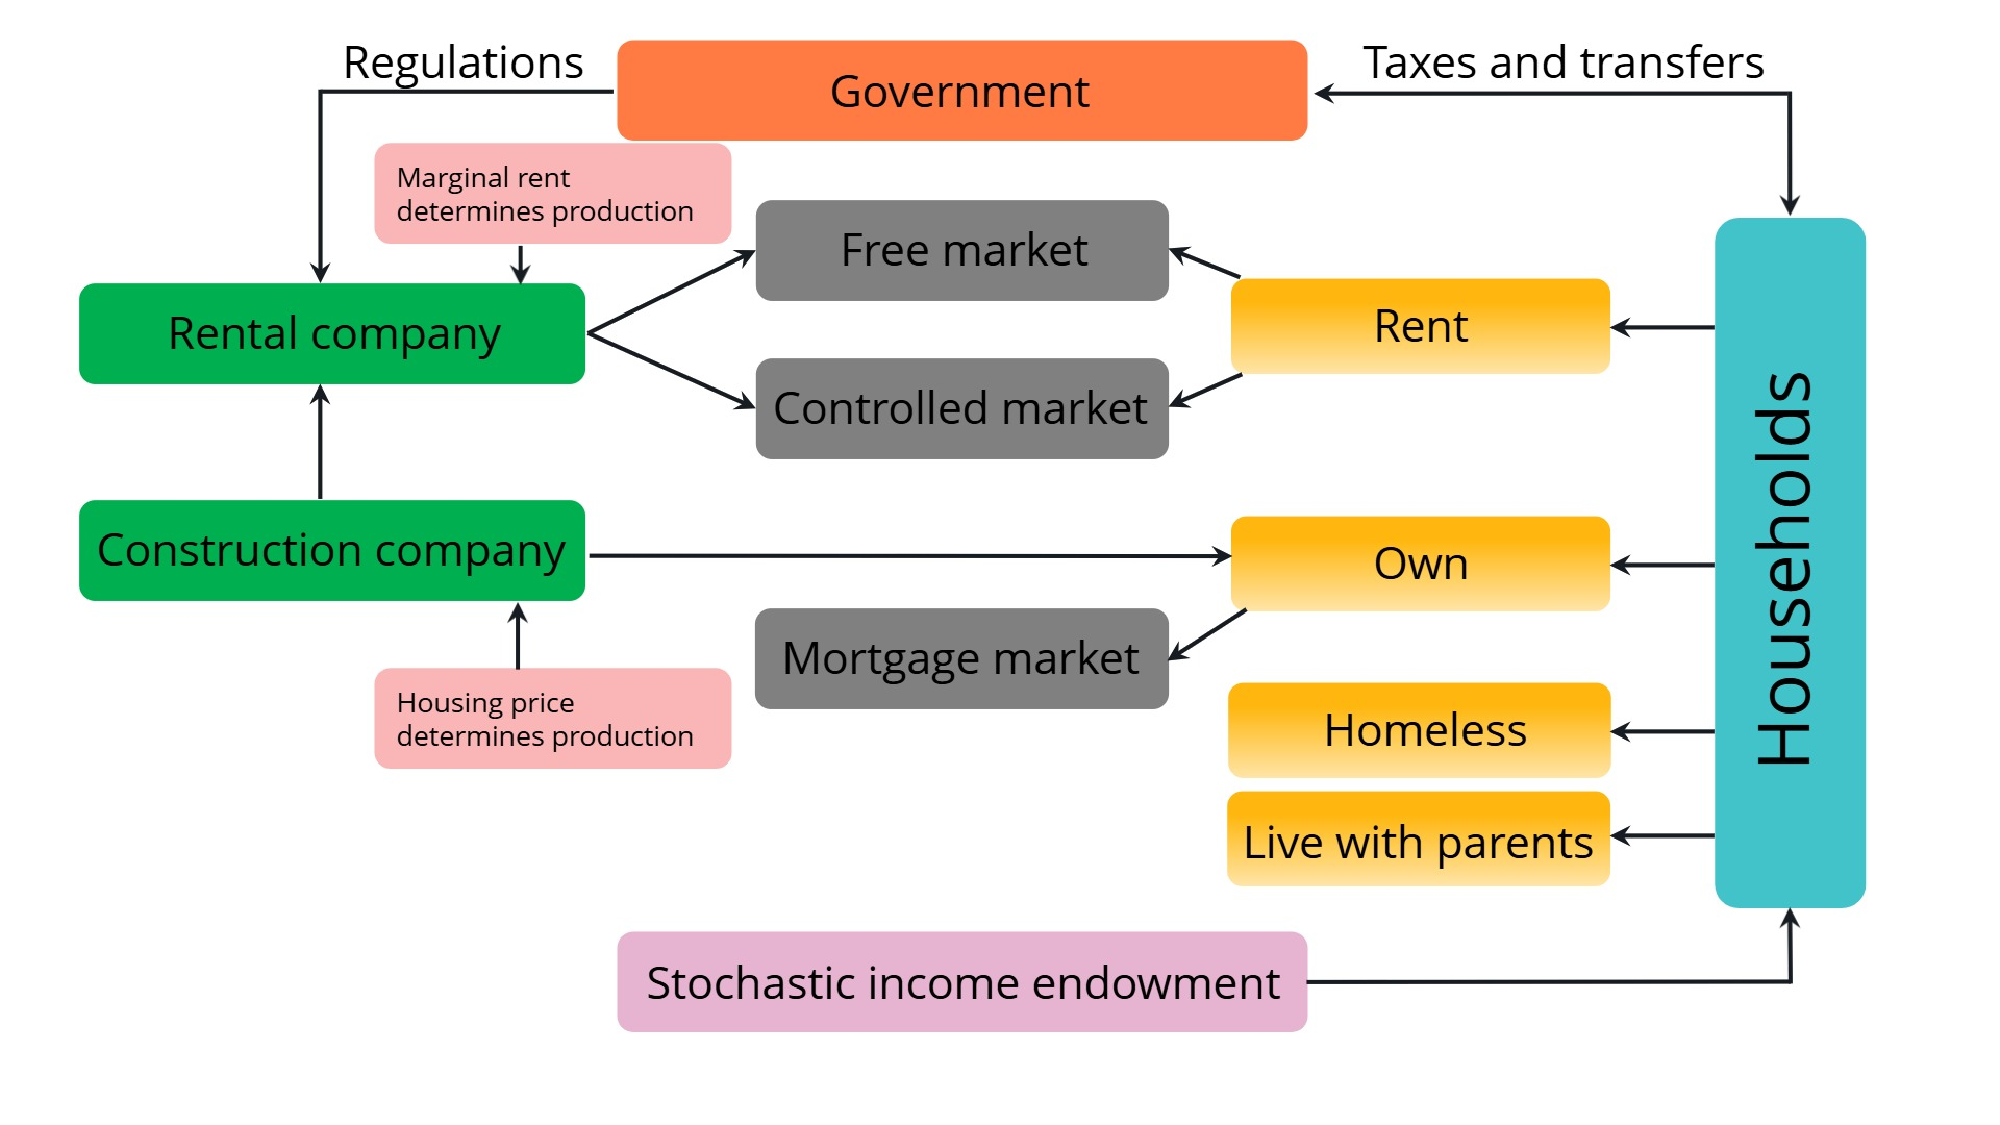
\includegraphics[width=0.9\textwidth]{figures_for_slides/model_flow_diagram.pdf}
\end{frame}

%%%%%%%%%%%%%%%%%%%%%%%%%
%%%%%%%%%%%%%%%%%%%%%%%%%
\begin{frame}{Model}{Household preferences and demographic structure}

Flow utility:
\begin{equation*}
    u_{j}(c,h)=\xi_{j}^{\sigma}\frac{\left(c^{1-\gamma} h(o,f,\iota)^{\gamma}\right)^{1-\sigma}}{1-\sigma},
\end{equation*}

\begin{itemize}
    \item $\xi_{j}$: equivalent household size scaling
    \item $c$: non-housing consumption, $h$: housing consumption, $o$: 1:=owner; 0:=renter
    \item $f$: 1:=rent in free market, 0:=rent in controlled market, $\iota$: number of years in unit
    \item $\gamma$: weight on housing consumption, $\sigma$: risk aversion
\end{itemize}

Warm glow:
\begin{equation*}
    \omega_{B}(q)=\mu \frac{q^{1-\sigma}}{1-\sigma}
\end{equation*}

\begin{itemize}
    \item $q$: household net wealth at death
\end{itemize}

\end{frame}

\begin{frame}{Model}{Demographic structure}

Overlapping generations of finitely-lived households:
\begin{itemize}
    \item Live from age $1$ to $J$ and die with certainty after $J$
    \item Work while $j<J_{R}$ and in retirement when $j\geq J_{R}$
\end{itemize}

\end{frame}

%%%%%%%%%%%%%%%%%%%%%%%%%
%%%%%%%%%%%%%%%%%%%%%%%%%

\begin{frame}{Model}{Household heterogeneity}
Households are heterogeneous in:
\begin{itemize}
    \item Age, $j \in \mathcal{N}$
    \item Financial wealth, $a \in \mathcal{R_{+}}$
    \item Housing tenure, $o \in \{0,1\}$; $0:=$renter, $1:=$owner
    \item Rental market in which they rent; $f \in \{0,1\}$, $0:=$controlled market, $1:=$free market
    \item Years in same unit, $\iota \in \mathcal{N}$
    \item Housing size, $h \in \mathcal{R_{++}}$; smallest rental $\underline{h}_{r}>0$, smallest owner-occupied $\underline{h}_{o}>\underline{h}_{r}$
    \begin{itemize}
        \item Homeless if $h=\underline{h}_{h}$
        \item Live with parents if $h=\underline{h}_{p}$; $\underline{h}_{h}<\underline{h}_{p}<\underline{h}_{r}$
    \end{itemize}
    \item Mortgage debt, $m \in \mathcal{R_{+}}$
    \item Idiosyncratic labor fixed effect, $\chi \in \mathcal{R_{++}}$
    \item Stochastic labor productivity, $e \in \mathcal{R_{++}}$
    \item $s$ to denote household state $(a,o,f,\iota,h,m,\chi,e)$
\end{itemize}

\end{frame}

%%%%%%%%%%%%%%%%%%%%%%%%%
%%%%%%%%%%%%%%%%%%%%%%%%%

\begin{frame}{Model}{Labor and capital income}

\begin{itemize}
    \item Labor income, $y_{\ell,j}(\chi,e)=\chi e \zeta_{j}$, for $j<J_{R}$ $\zeta_{j}$: deterministic age-dependent productivity
    \begin{itemize}
        \item Retirees receive pension, $y_{R}(\chi,e)$, where higher productivities receive higher pensions
        \item $e:$ follows Markov chain $\log e' = \rho_{e} \log e + \epsilon_{e},\quad \epsilon_{e}\sim N(0,\sigma_{e})$
    \end{itemize}
    \item Capital income, $y_{k}(a)=ar$
\end{itemize}
\end{frame}

%%%%%%%%%%%%%%%%%%%%%%%%%
%%%%%%%%%%%%%%%%%%%%%%%%%

\begin{frame}{Model}{Taxes}

\begin{itemize}
    \item Taxable income, $y^{x}_{j}(\chi,e,a)=y_{\ell,j}(\chi,e)+\nu y_{k}(a)$, $\nu$: taxable portion of capital income
    \item Progressive taxes, $y^{\tau}_{j}(\chi,e,a) = y^{x}_{j}(\chi,e,a)-\tau_{\ell}y^{x}_{j}(\chi,e,a)^{\psi}$, $\tau_{\ell}$: avg. tax, $\psi$: progressivity
    \item Proportional non-housing consumption tax rate, $\tau_{c}$
\end{itemize}

\end{frame}

%%%%%%%%%%%%%%%%%%%%%%%%%
%%%%%%%%%%%%%%%%%%%%%%%%%

\begin{frame}{Model}{Housing and tenure choice}

\begin{itemize}
    \item All housing depreciates at a rate $\delta_{h}$
    \item All housing is subject to a property tax rate $\tau_{p}$
\end{itemize}

\vspace{0.3cm}

\begin{itemize}
    \item Households can choose rent ($o=0$), own ($o=1$), or neither
    \item Households choosing neither can live with parents if $j\leq J_{p}$ or become homeless if $j>J_{p}$
\end{itemize}

\vspace{0.3cm}

\begin{itemize}
    \item Smallest rental unit available is $\underline{h}_{r}$ 
    \item Smallest owner-occupied unit available is $\underline{h}_{r}<\underline{h}_{o}$
    \item Those staying with parents live rent free, but receive reduced housing services $\underline{h}_{p}<\underline{h}_{r}$
    \item Homeless do not pay rent either, but receive further reduced housing services $\underline{h}_{h}<\underline{h}_{p}$
\end{itemize}

\end{frame}

\begin{frame}{Model}{Renters in controlled market}

Renters can choose to rent in controlled market $(f=0)$ or free market $(f=1)$ 
\begin{itemize}
    \item Renters choosing controlled market pay $\frac{p^{r}_{0}}{(1+\kappa_{1})^{\iota}} h$: 
    \begin{itemize}
        \item $p^{r}_{0}$: controlled market rent of new tenants
        \item $h$: initial housing choice (before it deteriorates)
        \item $\iota$: number of periods in same unit
        \item $\kappa_{1}$: rate of decline in real controlled rent with each additional period tenant remains in unit
    \end{itemize}
    \item However, landlords neglect unit $\rightarrow$ housing depreciates at rate $\kappa_{2}$: $h(\iota)=\frac{1}{(1+\kappa_{2})^{\iota}} h$
\end{itemize}

\end{frame}

\begin{frame}{Model}{Renters in free market}

\begin{itemize}
    \item Renters choosing free market pay $p^{r}_{1}h$, and landlords maintain their units
    \item But they risk shock, $z$, in subsequent period requiring additional payment of $z p^{r}_{1}h$
    \item $z$ is drawn from distribution $G(z)$, and can take positive or negative value
    \item Avg. free market rent is $\overline{p}^{r}_{1}=\int_\mathcal{Z}(1+z)p_{r,1}\mathrm{d}G(z)$
\end{itemize}

\end{frame}

\begin{frame}{Model}{Controlled vs. free market choices}
    \begin{columns}[T]
        \begin{column}{0.6\textwidth}  
            \caption{Qualitative depiction of rent path based on rental market choice and years in same rental}
            \hspace*{-1cm}
            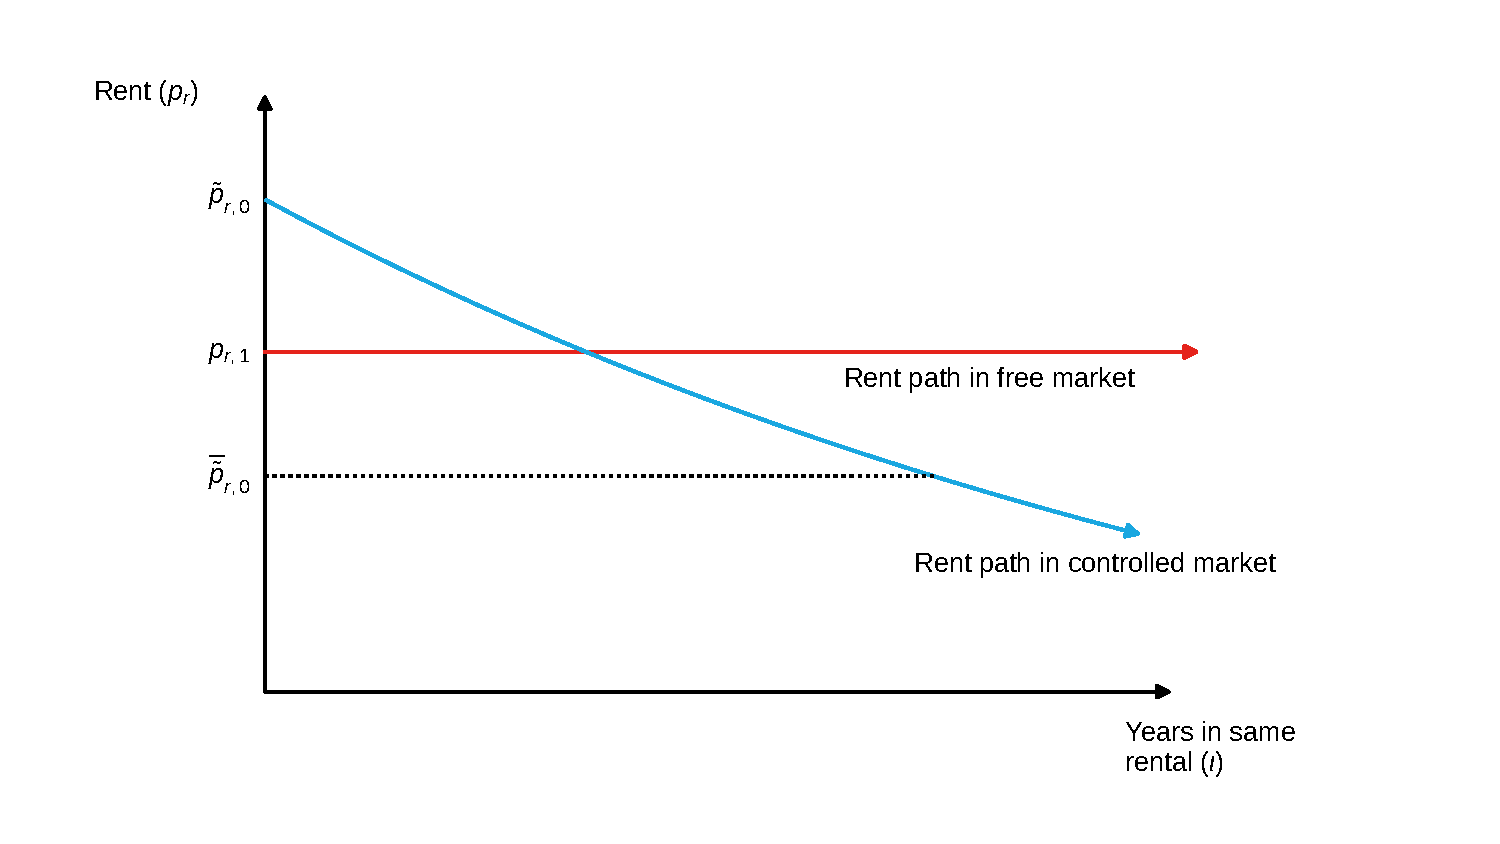
\includegraphics[width=1.35\textwidth]{figures/path_of_rent_diagram.pdf}
        \end{column}
        \begin{column}{0.4\textwidth}
            \begin{itemize}
            \item To clear markets, renters in controlled market pay initially more than in free market
                \begin{itemize}
                    \item Renters planning to buy quickly $\rightarrow$ sort to free market to avoid premium
                    \item Renters planning to remain renters long $\rightarrow$ pay premium and enjoy lower average rents in controlled market
                \end{itemize}
            \end{itemize}
        \end{column}
    \end{columns}
\end{frame}

\begin{frame}{Model}{Homeowners}

\begin{itemize}
    \item Offset housing depreciation each period
    \item Owners have access to long-term mortgages, $m$ \citep{rs-2023}
    \item At origination pay $\omega_{1}$ and must satisfy:
    \begin{itemize}
        \item LTV constraint $m \leq \lambda_{m,1}(ph) p h$
        \item GDS constraint $\frac{\tau_{p}ph+(r_{m}+\upsilon_{1})m}{y_{\ell,j}(e)+y_{k}(a)} \leq \lambda_{m,2}\left(\frac{m}{ph}\right)$
    \end{itemize}
    \item Pay at least $\upsilon_{1}m$ each period or incur cost of origination again
    \item Can pay up to $\upsilon_{2}>\upsilon_{1}$ without prepayment penalty
    \begin{itemize}
        \item Otherwise pay prepayment penalty: $\tau_{pp}=\omega_{2}\mbox{max}\left\{(1-\upsilon_{2})m-m',0\right\}$
    \end{itemize}
    \item Retirees cannot originate new mortgages
\end{itemize}

\end{frame}

%%%%%%%%%%%%%%%%%%%%%%%%%
%%%%%%%%%%%%%%%%%%%%%%%%%
\begin{frame}{Model}{Dynamic program}
\footnotesize
\begin{align}
  \label{eq:vf}
  V_{j}(s)=\max_{c,a',o',f',\iota',h',m'}\ \biggl\{u_{j}\left(c,h'(o',f',\iota')\right)+
  \indicator{j=J}\omega_{B}(q') + \indicator{j<J} \beta \mathbb{E}\biggl[V_{j+1}(s'|e,z)\biggl]\biggr\}
\end{align}
subject to
\begin{flalign}
  \begin{split} \label{eq:bc}
  & c(1+\tau_{c})+a'+(1-o')\left[(1-f')\frac{p^{r}_{0}}{(1+\kappa_{1})^{\iota'-1}}h'+f'p^{r}_{1}h'\right]+ fzp_{r,1}h + o'(ph'-m') +\\ & \quad o\left(ph\left(\tau_{p}+\delta_{h}\right)+r_{m}m\right)+\tau_{b}ph'(\mbox{purchase=1})+\tau_{s}ph(\mbox{sell=1})+ \omega_{1}(\mbox{new mortgage=1})+\\ & \quad \tau_{pp}(\mbox{prepayment penalty=1}) = \mbox{(after tax income from all sources)}+a+o(ph-m)
  \end{split} \\
  & f' \in \{0,1\} \hspace{0.2cm} \mbox{and} \hspace{0.2cm} h' \geq \underline{h}_{r} \hspace{0.2cm} \mbox{if} \hspace{0.2cm} o'=0, \hspace{0.2cm} h' \geq \underline{h}_{o} \hspace{0.2cm} \mbox{if} \hspace{0.2cm} o'=1 \hspace{0.2cm} \label{eq:rental_market_type} \\
  & h' = \underline{h}_{p} \hspace{0.2cm} \mbox{if} \hspace{0.2cm} j\leq J_{p} \hspace{0.2cm} \mbox{and live with parents}, \hspace{0.2cm} h' = \underline{h}_{h} \hspace{0.2cm} \mbox{if} \hspace{0.2cm} j> J_{p} \hspace{0.2cm} \mbox{and homeless},\label{eq:min_housing}\\
  & q' = a' + o'[ph'-m] \\
  & \mbox{Satisfy LTV \& GDS constraints if originating new mortgage}
\end{flalign}

Policy functions:
\begin{itemize}
    \item $c_{j}(s)$, $a'_{j}(s)$, $o'_{j}(s)$, $f'_{j}(s)$, $\iota'_{j}(s)$, $h'_{j}(s)$, and $m'_{j}(s)$
\end{itemize}

\end{frame}

%%%%%%%%%%%%%%%%%%%%%%%%%
%%%%%%%%%%%%%%%%%%%%%%%%%
\begin{frame}{Model}{Rental company (part 1)}
Rental company buys housing and rents them out:
\begin{align}\label{eq:rental_company_problem}
V(X)=\underset{X'_{0},X'_{1}} {\text{$\mbox{max} $}}\left\{\sum_{i=0}^{1} \overline{p}^{r}_{i}X'_{i}-\frac{\theta_{1}}{\theta_{2}}X'^{\theta_{2}}-p X'+p(1-\delta_{h}-\tau_{p})X+\frac{1}{1+r}V(X')\right\}.
\end{align}
subject to
\begin{align*}
& X'_{0}=\mbox{min}\{\underline{X}_{0},X'\}, \hspace{0.2cm} X'_{1} \geq 0, \hspace{0.2cm} X'=\sum^{1}_{i=0} X'_{i}
\end{align*}

\begin{itemize}
    \item $\underline{X'}_{0}$: amount of mandated controlled units; $X'_{1}$: supply on free market
    \item $\overline{p}^{r}_{1}$: avg. free market rent, which is also the marginal rent for rental company
    \item $\overline{p}^{r}_{0}$: avg. rent in controlled market
    \item $\theta_{1}$: avg. management cost; $\theta_{2} \geq 1$: convexity of cost of supplying more rental housing
\end{itemize}

\end{frame}

\begin{frame}{Model}{Rental company (part 2)}

\begin{itemize}
    \item Rental supply function:
    $X'^{*}=\left[\frac{1}{\theta_{1}}\left(\overline{p}^{r}_{1}-p\left(\frac{r+\delta_{h}+\tau_{p}}{1+r}\right)\right)\right]^{\frac{1}{\theta_{2}-1}}$
    \begin{itemize}
        \item When rental markets are fully controlled, avg. rents in controlled market $\overline{p}^{r}_{0}$ replace $\overline{p}^{r}_{1}$
        \item In eq'm $\overline{p}^{r}_{1}>\overline{p}^{r}_{0}$ $\rightarrow$ moving to full control reduces marginal rent and quantity supplied
    \end{itemize}
\end{itemize}

\end{frame}

%%%%%%%%%%%%%%%%%%%%%%%%%
%%%%%%%%%%%%%%%%%%%%%%%%%
\begin{frame}{Model}{Housing construction company}

\begin{itemize}
    \item Law of motion for housing $H'=(1-\delta_{h})H+I$:
    \begin{itemize}
        \item $H$: housing stock, $I$: new housing investment
    \end{itemize}
    \item Competitive company constructs new housing with technology, $TC(I)=\frac{\epsilon_{1}}{\epsilon_{2}}I^{\epsilon_{2}}$
    \begin{itemize}
        \item $p$: housing price; $\epsilon_{2}$: controls rental supply elasticity; $\epsilon_{1}$: scalar
    \end{itemize}
    \item Optimal investment: $I^{*}=\left(\frac{p}{\epsilon_{1}}\right)^{\frac{1}{\epsilon_{2}-1}}$
\end{itemize}

\end{frame}

\begin{frame}{Model}{Government}

Must balance budget each period; $G + \sum_{j=1}^J \int_\mathcal{S} \theta (\mbox{homeless=1})(s)\mathrm{d}\Psi(s)= \tau_p p H$
\begin{itemize}
    \item $G$: public good; picked in benchmark to clear budget; held fixed in counterfactuals
    \item $\theta$: cost to government per homeless (supports like health, justice, and housing systems)  
    \item Adjust $\tau_p$ in counterfactuals to clear budget
\end{itemize}

\end{frame}

\begin{frame}{Model}{Equilibrium definition}

A stationary eq'm in the model is:

\begin{itemize}
    \item a sequence of aggregate prices and quantities, $\left\{H',I,\{X'_{i},\overline{p}^{r}_{i}\}^{1}_{i=0},p\right\}$;
    \item value and policy functions, $\biggl\{V_{j}(\cdot),c_{j}(\cdot),a'_{j}(\cdot),o'_{j}(\cdot),f'_{j}(\cdot),\iota'_{j}(\cdot),h'_{j}(\cdot),m'_{j}(\cdot)\biggl\}_{j=1}^J$; and
    \item a sequence of measures, $\left\{\Psi_{j}(\cdot)\right\}_{j=1}^J$, that:
\end{itemize}
\begin{enumerate}
%\item all nominal prices rise at the rate of $i$, but real prices remain fixed;
\item solve household's dynamic problem subject to constraints;
\item solve rental company's problem subject to constraints;
\item satisfy construction company's first-order condition;
\item satisfy government's budget constraint;
\item clear housing market;
\item clear rental housing markets;
\item and satisfy laws of motion for the distribution of households
\end{enumerate}
    
\end{frame}

{\setbeamercolor{background canvas}{bg=black}
\begin{frame}{}

\centering \Large
\textcolor{white}{Calibration}
    
\end{frame}

}

%%%%%%%%%%%%%%%%%%%%%%%%%
%%%%%%%%%%%%%%%%%%%%%%%%%
\begin{frame}{Calibration}{External calibration (part 1)}

\begin{table}[p]
\footnotesize
\renewcommand{\arraystretch}{1.2}
\begin{center}
  %\caption{\centreing Assigned parameter values}
  %\label{tab:calibration}
\begin{tabular}{clcl}\toprule
Parameter & Description & Value & Source\\
\midrule
\multicolumn{4}{l}{\textit{(i) Externally demographic parameters}}\\
\midrule
$J$ & Lifespan & $60$ & Age range=26-85 \\
$J_{R}$ & Retirement age & $41$  & Retirement age=66 \\
$J_{p}$ & Maximum age household can live with parents & $9$ & \citet{rs-2023} \\
$\sigma$ & Risk aversion & 2 & Standard\\
$\{\xi_j\}_{j=1}^{J}$ & Equivalent household size scaling & Varies & Census (2016)\\
\bottomrule
\bottomrule
\end{tabular}
\end{center}
\normalsize
\end{table}


\end{frame}

\begin{frame}{Calibration}{External calibration (part 2)}

\begin{table}[p]
\footnotesize
\renewcommand{\arraystretch}{1.2}
\begin{center}
  %\caption{\centreing Assigned parameter values}
  %\label{tab:calibration}
\begin{tabular}{clcl}\toprule
Parameter & Description & Value & Source\\
\midrule
\multicolumn{4}{l}{\textit{(ii) Externally assigned labor productiity parameters}}\\
\midrule
$\rho_{e}$ & Labor productivity shock persistence & 0.9 & \citet{gkkoc} \\
$\rho_{\chi}$ & Inter-gen. labor fixed effect persistence  & 0.5 & \citet{gkkoc} \\
$\sigma_{\chi}$ & Inter-gen. labor fixed effect volatility & 0.309 & \citet{gkkoc} \\
$F(e,e'|b=1)$ & Increased prob. low labor shock & $1.2\times F(e,e'|b=0)$ & \citet{az-2024} \\
$\{\zeta_j\}_{j=1}^{R}$ & Lifecycle labor productivity & Varies & Census (2016) \\
$y_{R}(\chi,e)$ & Pension &  Varies & \citet{OECD-pension}\\
\bottomrule
\bottomrule
\end{tabular}
\end{center}
\normalsize
\end{table}


\end{frame}

\begin{frame}{Calibration}{External calibration (part 3)}

\begin{table}[p]
\footnotesize
\renewcommand{\arraystretch}{1.2}
\begin{center}
  %\caption{\centreing Assigned parameter values}
  %\label{tab:calibration}
\begin{tabular}{clcl}\toprule
Parameter & Description & Value & Source\\
\midrule
\multicolumn{4}{l}{\textit{(iii) Externally assigned tax parameters}}\\
\midrule
$\nu$ & Percent of capital income that is taxable & $50\%$ & Canada's tax code \\
$\tau_{c}$ & Non-housing consumption tax rate & $13\%$ & Ontario's HST \\
$\psi$ & Progressivity of labor income taxation & 0.897 & Census (2016) \\
$r$ & Interest rate & 2.77\% & \citet{bruneau-etal-2018} \\
\bottomrule
\bottomrule
\end{tabular}
\end{center}
\normalsize
\end{table}


\end{frame}

\begin{frame}{Calibration}{External calibration (part 4)}

\vspace{-0.5cm}
\begin{table}[p]
\footnotesize
\renewcommand{\arraystretch}{1.2}
\begin{center}
  %\caption{\centreing Assigned parameter values}
  %\label{tab:calibration}
\begin{tabular}{clcl}\toprule
Parameter & Description & Value & Source\\
\midrule
\multicolumn{4}{l}{\textit{(iv) Externally assigned housing parameters}}\\
\midrule
$\left\{z\right\}_{\mathbb{Z}}$ & Free-market rent shocks & Varies & RMS (1992-2016) \\
$G(z)$ & Free-market rent shock prob. & Varies & RMS (1992-2016) \\
$\kappa_{1}$ & Real rent decrease if staying in unit & 1.365\% & Census (2016) \& RMS (1992-2016) \\
$\kappa_{2}$ & Controlled unit deterioration & 0.55\% & \citet{murray_et_al-1991} \\
$\delta_h$ & Housing depreciation & 0.6\% & \citet{rosenthal-2014} \\
$\theta_{b}$ & Cost per homeless hhld & 0.83 $\times$ avg. inc. & Homelessness Hub \& City of Toronto\\
$\tau_p$ & Property tax rate & 0.44\% & City of Toronto \& PSAD (1992-2016) \\
$\tau_{b}$ & Buying cost & 2\% & \citet{gm-2003} \\
$\tau_{s}$ & Selling cost & 6\% & \citet{gm-2003} \\
$\epsilon_2$ & Elasticity of housing investment & 1.89 & \citet{piaxao-2021} \\
$\overline{p}^{r}/p$ & Avg. rent/housing price & 5.24\% & RMS (2016) \& CREA (2016) \\
\bottomrule
\bottomrule
\end{tabular}
\end{center}
\normalsize
\end{table}


\end{frame}

\begin{frame}{Calibration}{External calibration (part 5)}

\begin{table}[p]
\footnotesize
\renewcommand{\arraystretch}{1.2}
\begin{center}
  %\caption{\centreing Assigned parameter values}
  %\label{tab:calibration}
\begin{tabular}{clcl}\toprule
Parameter & Description & Value & Source\\
\midrule
\multicolumn{4}{l}{\textit{(v) Externally assigned mortgage parameters}}\\
\midrule
$\lambda_{m,1}(ph)$ & Maximum LTV ratio & [80\%,90\%,95\%] & Canada's banking regulations \\
$\lambda_{m,2}$ & Maximum PTI ratio & 39\% & Canada's banking regulations \\
$\omega_{2}$ & Mortgage origination cost & 0.68\% of avg. income & Census (2016) \& CMHC \\
$\omega_{3}$ & Prepayment penalty & 3 months' interest & Canadian banking practices \\
$\upsilon_{1}$ & Avg. fraction of mortgage paid & 1.7\% & \citet{kkk-2021} \\
$\upsilon_{2}$ & Threshold for prepayment penalty & 18.8\% & Canadian banking practices \\
$\Delta_{m}$ & Mortgage premium & 0.19\% & Mortgage-bond spread \\
\bottomrule
\bottomrule
\end{tabular}
\end{center}
\normalsize
\end{table}


\end{frame}

\begin{frame}{Calibration}{Internal calibration}
\vspace{-0.1cm}

\vspace{-0.6cm}
\begin{table}[p]
\footnotesize
\renewcommand{\arraystretch}{1.2}
\begin{center}
  %\caption{\centreing Assigned parameter values}
  %\label{tab:calibration}
\begin{tabular}{clcl}\toprule
Parameter & Description & Value & Source\\
\midrule
$\beta$ & Discount factor & 0.961 & Mortgages/housing value=21.5\% \\
$\gamma$ & Weight on housing preferences & 0.211 & Rent/income=22.5\% \\
$\mu$ & Strength of bequest motive & 160 & Bequests/net wealth=2.2\% \\
$\tau_{\ell}$ & Avg. income tax rate & 0.877 & Avg. income tax=19.6\% \\
$\sigma_{e}$ & Labor productivity shock volatility & 0.140 & Labor income Gini coefficient=0.49 \\
$\theta_{2}$ & Convexity of rental costs & 9.939 & Tax incidence of renters=12\% \\
$\theta_{1}$ & Managerial cost/avg. free rent & $\frac{\theta_{1}X^{\theta_{2}-1}}{\overline{p}_{r,1}}=40\%$ & Avg. free rent/housing price=5.82\% \\
$p_{r,0}$ & Initial rent in controlled unit & $\frac{p_{r,0}}{\overline{p}_{r,1}}=1.062$ & Renters in controlled market=71\% \\
$\underline{h}_{r}$ & Smallest rental unit & $0.585 \times \hat{h}_{o}$  & Renters with rent/income$>$0.5=15.4\% \\
$\underline{h}_{o}$ & Smallest owned-house & $6.17 \times \frac{\hat{h}_{o}}{\mbox{avg. inc.}}$ & Homeownership rate=66.5\% \\
$\underline{h}_{p}$ & Housing services if with parents & $0.27 \times \underline{h}_{r}$ & Young living with parents=22.3\% \\
$\underline{h}_{h}$ & Housing services if homeless & $0.062 \times \underline{h}_{r}$ & Homelessness rate=0.26\% \\
\bottomrule
\bottomrule
\end{tabular}
\end{center}
\normalsize
\end{table}


\end{frame}

{\setbeamercolor{background canvas}{bg=black}
\begin{frame}{}

\centering \Large
\textcolor{white}{Model perfomance}
    
\end{frame}

}

\begin{frame}{Model performance}{Non-targeted moments - aggregates (part 1)}

\begin{table}[p]
\footnotesize
%\caption{\centreing Non-targeted moments}
%\label{tab:aggregate_non_targreted_statistics}
\renewcommand{\arraystretch}{1.2}
\begin{center}
\begin{tabular}{lcclcl}\toprule
Statistic & Model & Data & Source\\
\midrule
\multicolumn{4}{l}{\textit{(a) Aggregate statistics}}\\
Avg. owned-house value/Avg. hhld inc. & 6.17 & 5.78 & Census (2016) \& SFS (2019) \\
Owners with mortgage & 45\% & 63\% & SFS (2019) \\
\multicolumn{4}{l}{\textit{(a) Rental markets}}\\
Avg. rental/avg. owner-occupied & 0.56 & 0.66 & \citet{chatterjee-eyigungor-2015} \\
Avg. free rent/avg. controlled rent & 1.03 & -- & -- \\
Avg. inc. in free/avg. inc. in controlled & 2.7\% & 18.9\% & Census (2016) \\
\bottomrule
\bottomrule
\end{tabular}
\end{center}
\normalsize
\end{table}


\end{frame}

\begin{frame}{Model performance}{Non-targeted moments - aggregates (part 2)}

\begin{table}[p]
\footnotesize
%\caption{\centreing Non-targeted moments}
%\label{tab:aggregate_non_targreted_statistics}
\renewcommand{\arraystretch}{1.2}
\begin{center}
\begin{tabular}{lcclcl}\toprule
Statistic & Model & Data & Source\\
\midrule
\multicolumn{4}{l}{\textit{(b) Wealth distribution}}\\
Top 1\% & 4\% & 14\% & \rdelim\}{5}{16pt}\multirow{5.2}{*}{SFS (2019)} \\
Top 10\% & 27\% & 49\% \\
Top 20\% & 47\% & 67\% \\
Bottom 50\% & 14\% & 7\% \\
Wealth Gini & 0.49 & 0.65 \\
\bottomrule
\bottomrule
\end{tabular}
\end{center}
\normalsize
\end{table}


\end{frame}

\begin{frame}{Model Performance}{Non-targeted moments - lifecycle}
  \centering
     \includegraphics[width=0.9\textwidth]{figures/lifecycle.pdf}
\end{frame}

\begin{frame}{Model performance}{Non-targeted moments - rent to income distribution}
  \centering
     \includegraphics[width=0.65\textwidth]{figures/rent_income_cdf.pdf}
    \begin{itemize}
        \item $(0.1,0.0)$ $-->$ no renters in model spend below 10\% of their income on housing
        \item $(0.5,0.85)$ $-->$ 15\% of renters in model spend over 50\% of their income on housing
    \end{itemize}
\end{frame}

\begin{frame}{Model performance}{Non-targeted moments - tenure by income quintile for working-age households}
  \centering     \begin{table}[p]
\footnotesize
\renewcommand{\arraystretch}{1.2}
\begin{center}
%\caption{\centreing Tenure by labor productivity in benchmark}
%\label{tab:tenure_by_labor_productivity}
\begin{tabular}{lccccccc}
\toprule
Rental market/Income quintile & Lowest & Second & Third & Fourth & Highest\\ 
\midrule
\multicolumn{6}{l}{\textit{(a) Data}}\\
Renters in controlled market (\%) & 42.90 & 28.90 & 17.50 &	9.10 & 4.10\\
Renters in free market (\%) & 15.80 & 10.60 & 8.00 & 5.40 & 3.50 \\
\multicolumn{6}{l}{\textit{(b) Baseline's benchmark (tenancy control)}}\\
Renters in controlled market (\%) & 43.09 & 34.67 & 10.36 & 16.80 & 8.33 \\
Renters in free market (\%) & 1.71 & 2.77 & 21.72 & 19.96 & 9.95 \\
\bottomrule
\end{tabular}
\end{center}
\normalsize
\end{table}

\end{frame}

%%%%%%%%%%%%%%%%%%%%%%%%%
%%%%%%%%%%%%%%%%%%%%%%%%%

{\setbeamercolor{background canvas}{bg=black}
\begin{frame}{}

\centering \Large
\textcolor{white}{Experiments}
    
\end{frame}

}

\begin{frame}{Experiments}{Overview}

We conduct 4 long-run experiments comparing them to benchmark:
\begin{itemize}
    \item Unit control
    \item Full decontrol
    \item Full tenancy control
    \item Welfare-maximizing degree of rent control in long-run
    \begin{itemize}
        \item Maximize ex-ante expected utility of newborns \citep{conesa-et-al,gkkoc}
    \end{itemize}
\end{itemize}

\vspace{0.5cm}

In all our experiments, we:
\begin{itemize}
    \item Balance government budget with property taxes
    \item Keep rest of tax system fixed
\end{itemize}
    
\end{frame}

\begin{frame}{Experiments}{Measure of rents}

\begin{enumerate}
    \item \underline{Free market rent}: rent in free market
    \item \underline{Avg. controlled rent}: avg. rent in controlled market
    \item \underline{Rent of new tenants}: rent new tenants pay when moving into a rental unit
    \item \underline{Avg. rent}: weighted avg. of rents in controlled and free markets
    \item \underline{Marginal rent}: rent that rental company receives if it supplied an additional rental unit
    \begin{itemize}
        \item When free markets operate, marginal rent is free market rent
        \item When all rental units are controlled, marginal rent is avg. rent in controlled market
    \end{itemize}
\end{enumerate}

\end{frame}

{\setbeamercolor{background canvas}{bg=black}
\begin{frame}{}

\centering \Large
\textcolor{white}{Experiment 1: Replacing tenancy control with unit control}
    
\end{frame}

}

\begin{frame}{Experiments}{Experiment 1: Unit control model differences}

    \begin{itemize}
    \item Households “wake-up" to encounter a random shock, $\eta \in\{0,1\}$
    \item With probability $\pi$, $\eta=1$; otherwise, it equals 0
    \item Households drawing $\eta=1$ can rent in controlled rental market in that period
    \begin{itemize}
        \item Once in controlled market, can stay in their unit irrespective of subsequent realizations of $\eta$
        \item Upon vacating unit, re-entry into controlled market requires another realization of $\eta=1$
    \end{itemize}
    \item Households drawing $\eta=0$ cannot rent in controlled rental market in that period
    \end{itemize}

\end{frame}

\begin{frame}{Experiments}{Experiment 1: Unit control experiment set up}

    \begin{itemize}
    \item Replace tenancy control with unit control
    \item Set controlled rent under unit control to equal average controlled rent in benchmark
    \item Pick $\pi$ such that proportion of rental market under control equals proportion in benchmark
    \item Real rent decrease, $\kappa_{1}$, equals unit deterioration rate, $\kappa_{2}$ $\rightarrow$ constant adjusted real rent
    \end{itemize}

\end{frame}

\begin{frame}{Experiments}{Experiment 1: Unit control, unit allocation outcomes}

\centering
     \begin{table}[p]
\footnotesize
\renewcommand{\arraystretch}{1.2}
\begin{center}
%\caption{\centreing Tenure by labor productivity in benchmark}
%\label{tab:tenure_by_labor_productivity}
\begin{tabular}{lccccccc}
\toprule
Rental market/Income quintile & Lowest & Second & Third & Fourth & Highest\\ 
\midrule
\multicolumn{6}{l}{\textit{(a) Data}}\\
Renters in controlled market (\%) & 42.90 & 28.90 & 17.50 &	9.10 & 4.10\\
Renters in free market (\%) & 15.80 & 10.60 & 8.00 & 5.40 & 3.50 \\
\multicolumn{6}{l}{\textit{(b) Baseline's benchmark (tenancy control)}}\\
Renters in controlled market (\%) & 43.09 & 34.67 & 10.36 & 16.80 & 8.33 \\
Renters in free market (\%) & 1.71 & 2.77 & 21.72 & 19.96 & 9.95 \\
\multicolumn{6}{l}{\textit{(c) Unit control model}}\\
Renters in controlled market (\%) & 34.69 & 28.43 & 19.27 & 18.41 & 9.47 \\
Renters in free market (\%) & 9.66 & 8.03 & 15.85 & 16.65 & 7.85\\
\bottomrule
\end{tabular}
\end{center}
\normalsize
\end{table}


\begin{itemize}
    \item Fewer controlled units go to low-income households $\rightarrow$ misallocation $\uparrow$
    \item Lotteries exclude low-income households more than premium under tenancy control
\end{itemize}

\end{frame}

\begin{frame}{Experiments}{Experiment 1: Unit control diagram}

\begin{columns}[T]
\begin{column}{0.5\textwidth}
\hspace*{-0.7cm}
\includegraphics[width=1.2\textwidth]{figures/unit_control_diagram.pdf}
\end{column}
\begin{column}{0.49\textwidth}
    \vspace{-0.75cm}
    \begin{itemize}
    \item Immediate rent discounts under unit control, taking 11 years in benchmark, spur rental demand of lucky renters (intensive margin)
    \item But, no further discounts from staying long $\rightarrow$ rental demand $\downarrow$ (extensive margin) $\rightarrow$ overall free-market rents $\uparrow$ (2.4\%) 
    \item HO $\uparrow$ house prices $\uparrow$ (0.4\%) $\rightarrow$ cost to supply rental housing $\uparrow$ $\rightarrow$ rental supply $\downarrow$
    \item Fewer low-income hhlds in controlled market and free-market rent $\uparrow$ $\rightarrow$ homelessness $\uparrow$ (16.3\%)
    \end{itemize}
\end{column}

\end{columns}

\end{frame}

\begin{frame}{Experiments}{Experiment 1: Unit control, distributional outcomes}

\begin{table}[p]
\footnotesize
\renewcommand{\arraystretch}{1.2}
\begin{center}
%\caption{\centreing Newborns' distributional impact by labor productivity (full deregulation relative to full rent control)}
%\label{tab:distributional_impact}
\begin{tabular}{lcccccc}
\toprule
Statistic & Experiment & Lowest & 2nd & 3rd & 4th & Highest\\ 
\midrule
%\multicolumn{8}{l}{\textit{(a) Full decontrol}}\\
Welfare effect ($\% \Delta$) & Unit control & -0.06 & -0.05 & -0.07 & -0.08 & 
-0.05 \\
\bottomrule
\bottomrule
\end{tabular}
\end{center}
\normalsize
\end{table}


\begin{itemize}
    \item Low-income lose $\rightarrow$ fewer under control \& higher free-market rent$>$immediate discounts
    \item Middle- and high-income lose $\rightarrow$ higher house prices and free market rents
    \item Partial eq'm exercise keeping free market rent at benchmark $\rightarrow$ slight welfare improvement
\end{itemize}

\end{frame}

{\setbeamercolor{background canvas}{bg=black}
\begin{frame}{}

\centering \Large
\textcolor{white}{Experiment 2: Completely removing any form of rent control}
    
\end{frame}

}

\begin{frame}{Experiments}{Experiment 2: Full decontrol diagram}

\begin{columns}[T]
\begin{column}{0.55\textwidth}
\hspace*{-0.7cm}
\includegraphics[width=1.2\textwidth]{figures/full_decontrol_diagram.pdf}
\end{column}
\begin{column}{0.4\textwidth}
    \vspace{-0.5cm}
    \begin{itemize}
    \item No premium for new tenants $\rightarrow$ demand $\uparrow$ (intensive margin)
    \item But, no tenancy control $\rightarrow$ incentive to rent $\downarrow$ $\rightarrow$ demand $\downarrow$ (extensive margin)
    \item HO $\uparrow$ $\rightarrow$ house prices $\uparrow$ (0.48\%) $\rightarrow$ rental supply $\downarrow$ $\rightarrow$ free-market rent $\uparrow$ (0.1\%)
    \item Households exposed to risk they want to avoid + rents $\uparrow$ + house prices prices $\uparrow$ $\rightarrow$ homelessness $\uparrow$ (32\%) and welfare $\downarrow$ (0.3\%) 
    \end{itemize}
\end{column}

\end{columns}

\end{frame}

{\setbeamercolor{background canvas}{bg=black}
\begin{frame}{}

\centering \Large
\textcolor{white}{Experiment 3: Regulating full rental market using tenancy control}
    
\end{frame}

}

\begin{frame}{Experiments}{Experiment 3: Full tenancy control diagram}

\begin{columns}[T]
\begin{column}{0.55\textwidth}
\hspace*{-0.6cm}
\includegraphics[width=1.18\textwidth]{figures/full_tenancy_control_diagram.pdf}
\end{column}
\begin{column}{0.48\textwidth}
    \vspace{-1.5cm}
    \begin{itemize}
    \item Free-market benchmark renters pay premium in controlled market $\rightarrow$ rental demand $\downarrow$ (intensive margin) 
    \item More stay in rental market $\rightarrow$ rental demand $\uparrow$ (extensive margin)
    \item HO $\downarrow$ $\rightarrow$ house prices $\downarrow$ (0.4\%) $\rightarrow$ rental supply $\uparrow$
    \item Avg. controlled rent is now rental company's marginal rent (instead of free-market rent) $\rightarrow$  avg. controlled rent must rise to supply benchmark quantity $\rightarrow$ avg. controlled rent $\uparrow$ (0.7\%) even though quantity supplied $\downarrow$ (0.6\%) 
    \item No free-market choice $\rightarrow$ welfare $\downarrow$ (.02\%) 
    \item No rent risk $\rightarrow$ homelessness $\downarrow$ (2\%) 
    \end{itemize}
\end{column}

\end{columns}

\end{frame}


{\setbeamercolor{background canvas}{bg=black}
\begin{frame}{}

\centering \Large
\textcolor{white}{Experiment 4: Welfare-maximizing share of market under tenancy control}
    
\end{frame}

}

\begin{frame}{Experiments}{Experiment 4: Welfare-maximizing degree of tenancy control}

Trade-offs in controlling rental market
\begin{itemize}
    \item Too little control $\rightarrow$ premia on controlled units $\uparrow$ $\rightarrow$ hurt low-income households
    \item Too much $\rightarrow$ free-market rent $\uparrow$ $\rightarrow$ divert to controlled market $\rightarrow$ hurt those in free market
\end{itemize}

\vspace{0.3cm}

\begin{itemize}
    \item Optimal control is 65\% (benchmark is about 70\%)
\end{itemize}

\end{frame}

{\setbeamercolor{background canvas}{bg=black}
\begin{frame}{}

\centering \Large
\textcolor{white}{Conclusion and discussion}
    
\end{frame}

}

%%%%%%%%%%%%%%%%%%%%%%%%%
%%%%%%%%%%%%%%%%%%%%%%%%%
\begin{frame}{Discussion}{Key takeaways}

Shortages:
\begin{itemize}
    \item Unit control $\rightarrow$ caps rent at unit level $\rightarrow$ shortages
    \item Tenancy control $\rightarrow$ caps rents during tenancy $\rightarrow$ no shortages
\end{itemize}

\vspace{0.1cm}

Misallocation:
\begin{itemize}
    \item Unit control $\rightarrow$ random assignment of controlled units $\rightarrow$ misallocation
    \item Tenancy control $\rightarrow$ premium allocates controlled units $\rightarrow$ better allocation, but....
    \item Min. rental size $\rightarrow$ premium may shut out highest willingness to pay $\rightarrow$ misallocation $\uparrow$?
\end{itemize}

\vspace{0.1cm}

Main results:
\begin{itemize}
    \item Unit control $\rightarrow$ welfare $\downarrow$, homelessness $\uparrow$, misallocation $\uparrow$ 
    \item Welfare-maximizing degree of tenancy control is 65\%
    \item Full decontrol and full tenancy control reduce welfare compared to benchmark
\end{itemize}

\end{frame}

\begin{frame}{Discussion}{Future research}
 
Future research could focus on:
\begin{itemize}
    \item Rent control and evictions
    \begin{itemize}
        \item Tenancy control encourages evictions relative to unit control. How does that impact welfare?
    \end{itemize}
    \item Rent control and endogenous labor supply
    \begin{itemize}
        \item How do rent control policies interact with labor supply and GDP?
    \end{itemize}
\end{itemize}
 
\end{frame}

{\setbeamercolor{background canvas}{bg=black}
\begin{frame}{}

\centering \Large
\textcolor{white}{References}
    
\end{frame}

}

\bibliographystyle{aer}
\bibliography{reference_files/bib}

\end{document}
